\documentclass[proposal.tex]{subfiles} 


\begin{document}

\section{Prototype 1}{\label{proto1}}

\subsection{About this chapter}
This chapter throws light on what \progLang{Prolog} does to resolve a given query via \textit{unification} and this can be replicated in
the host language along with the challenges.  

This chapter discusses the aspects of opening a language while preserving the original structure of a closed recursive structure in 
\progLang{Haskell}. Also discussed are the issues related to customizing certain aspects such as meta-syntactic variables.

\subsection{How Prolog works ?}
Looking at how \progLang{Prolog} works \cite{webiste:learnprolognow}.

Most \progLang{Prolog} distributions have three types of terms:
\begin{enumerate}
\item Constants.

\item Variables.

\item Complex terms.
\end{enumerate}

Two terms can be unified if they are the same or the variables can be assigned to terms such that the resulting terms are equal.

The possibilities could be,
\begin{enumerate}
\item If term1 and term2 are constants, then term1 and term2 unify if and only if they are the same atom, or the same number.

\item If term1 is a variable and term2 is any type of term, then term1 and term2 unify, and term1 is instantiated to term2 . Similarly, if 
term2 is a variable and term1 is any type of term, then term1 and term2 unify, and term2 is instantiated to term1 . (So if they are both 
variables, they’re both instantiated to each other, and we say that they share values.)

\item If term1 and term2 are complex terms, then they unify if and only if:

\begin{enumerate}
\item They have the same functor and arity, and

\item all their corresponding arguments unify, and

\item the variable instantiations are compatible.
\end{enumerate}

\item Two terms unify if and only if it follows from the previous three clauses that they unify.
\end{enumerate} 

For example,

\begin{minted}[linenos]{prolog}
append([],L,L). 
append([H|T],L2,[H|L3])  :-  append(T,L2,L3).
\end{minted}


\begin{figure}[h]
\centering
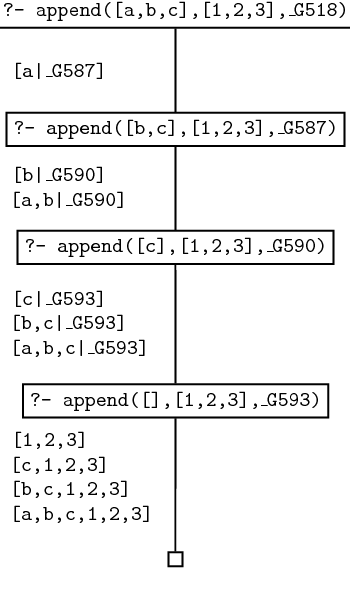
\includegraphics[scale = 0.5]{PrologAppendWorking.png}
\caption{Trace for append \cite{webiste:learnprolognowappend}}
\label{fig:Trace for append}
\end{figure}  

\begin{comment}
This chapter looks into solving the issue of conflicting type systems of the languages in question. \progLang{Haskell} is a strong 
statically typed language requiring type signature for programming constructs at compile time while \progLang{Prolog} is strong dynamically 
typed which lets through untyped programs. This prototype throws light on the process of tackling the issues involved in creating 
a data type to replicate the target language type system while conforming to the host language restrictions and also utilizing the 
benefits.       
\end{comment}

\subsection{What we do in this Prototype}
This prototype throws light on the process of tackling the issues involved in creating 
a data type to replicate the target language type system while conforming to the host language restrictions and also utilizing the 
benefits. 


We have a \progLang{Prolog} like language in \progLang{Haskell} defined via \textit{data}.

The language defined is recursive in nature. 

We convert it into a non recursive data type.


  


\subsection{Creating a data type}

A type system consists of a set of rules to define a "type" to different constructs in a programming language such as variables, functions 
and so on. A static type system requires types to be attached to the programming constructs before hand which results in finding errors at 
compile time and thus increase the reliability of the program. The other end is the dynamic type system which passes through code which 
would not have worked in former environment, it comes of as less rigid.

The advantages of static typing \cite{meijer2004static}
\begin{enumerate}
\item Earlier detection of errors
\item Better documentation in terms of type signatures
\item More opportunities for compiler optimizations
\item Increased run-time efficiency
\item Better developer tools 
\end{enumerate}          

For dynamic typing
\begin{enumerate}
\item Less rigid
\item Ideal for prototyping / unknown / changing requirements or unpredictable behaviour 
\item Re-usability  
\end{enumerate}

\paragraph{Transitional paragraph}
An ideal case would would be something that is ........ dont know what to write


To start with, replicating the single type "term" in \progLang{Prolog} one must consider the distinct constructs it can be associated to 
such as complex structures (for example predicates, clauses etc.), don't cares, cuts, variables and so on.

Consider the language below,

\begin{minted}[linenos]{haskell}	
data VariableName = VariableName Int String
      deriving (Eq, Data, Typeable, Ord)
data Atom         = Atom      !String
                  | Operator  !String
      deriving (Eq, Ord, Data, Typeable)
data Term = Struct Atom [Term]
          | Var VariableName
          | Wildcard
          | PString   !String
          | PInteger  !Integer
          | PFloat    !Double
          | Flat [FlatItem]
          | Cut Int
      deriving (Eq, Data, Typeable)
data Clause = Clause { lhs :: Term, rhs_ :: [Goal] }
            | ClauseFn { lhs :: Term, fn :: [Term] -> [Goal] }
      deriving (Data, Typeable)
type Program = [Sentence]
type Body    = [Goal]
data Sentence = Query   Body
              | Command Body
              | C Clause
      deriving (Data, Typeable)
\end{minted}

Even though \textit{Term} has a number of constructors the resulting construct has a single type. Hence, a function would still be untyped 
/ singly typed,
\begin{minted}{haskell}
append :: [Term] -> [Term] -> [Term]
\end{minted} 

The above data type is recursive as seen in the constructor,
\mint{haskell}|Struct Atom [Term]|

One of the issues with the above is that it is not possible to distinguish the structure of the data from the data type itself 
\cite{sheard2004two}. Consider the following, a reduced version of the above data type,

\begin{minted}[linenos]{haskell}
type Atom         = String
data VariableName = VariableName Int String
      deriving (Eq, Data, Typeable, Ord)
data Term = Struct Atom [Term]
          | Var VariableName
          | Wildcard -- Don't cares 
          | Cut Int
      deriving (Eq, Data, Typeable)
\end{minted}

Also one cannot create Quantifiers plus logic 

To split a data type into two levels, a single recursive data type is replaced by two related data types. Consider the following,
\begin{minted}[linenos]{haskell}
data FlatTerm a = 
		 Struct Atom [a]
	|	Var VariableName
	|	Wildcard
	|	Cut Int deriving (Show, Eq, Ord)
\end{minted}

One result of the approach is that the non-recursive type \textit{FlatTerm} is modular and generic as the structure "FlatTerm" is separate 
from it's type which is "a". Simply speaking we can have something like 
\mint{haskell}|FlatTerm Bool|

and a generic fuinction like,
\mint{haskell}|map :: (a -> b) -> FlatTerm a -> FlatTerm b|


\subsection{Working with the language}
Creating instances,
\begin{minted}[linenos]{haskell}
instance Functor (FlatTerm) where
	fmap = T.fmapDefault
instance Foldable (FlatTerm) where
 	foldMap = T.foldMapDefault
instance Traversable (FlatTerm) where
  	traverse f (Struct atom x)	=	Struct atom <$> 
  				sequenceA (Prelude.map f x)
  	traverse _ (Var v)	=	pure (Var v)
  	traverse _ Wildcard	=	pure (Wildcard)
  	traverse _ (Cut i)	= 	pure (Cut i)
instance Unifiable (FlatTerm) where
	zipMatch (Struct al ls) (Struct ar rs) = 
		if (al == ar) && (length ls == length rs) 
			then Struct al <$> 
				pairWith (\l r -> Right (l,r)) ls rs  		
			else Nothing
	zipMatch Wildcard _ = Just Wildcard
	zipMatch _ Wildcard = Just Wildcard
	zipMatch (Cut i1) (Cut i2) = if (i1 == i2) 
		then Just (Cut i1) 
		else Nothing
instance Applicative (FlatTerm) where
	pure x = Struct "" [x] 
	_ <*> Wildcard	= 	Wildcard
	_ <*> (Cut i) 	= 	Cut i
	_ <*> (Var v)	=	(Var v)
	(Struct a fs) <*> (Struct b xs) = Struct (a ++ b) [f x | f <- fs, x <- xs] 
\end{minted}

After flattening do fixing,
 

Opening up the language somehow so as to accommodate your own variables.







\subsection{Black box}

hello
\end{document}